\chapter{Phương pháp chèn hình ảnh}

Trong một luận văn hay báo cáo, các hình ảnh được sử dụng rất nhiều. Việc chèn hình ảnh tuy đơn giản nhưng cần sử dụng nhiều kỹ thuật. Chương này trình bày các cách chèn hình ảnh từ đơn giản tới phức tạp.

\section{Chèn hình ảnh đơn điệu}

Chèn hình ảnh đơn điệu nghĩa là chỉ chèn một hình ảnh cơ bản, có cú pháp latex như sau:

\begin{lstlisting}[language={[LaTeX]TeX}, caption={Chèn một hình ảnh vào báo cáo}, label={lst:figure}]
\begin{figure}
    \centering
    \includegraphics[scale=0.7]{chapter1/figure-url.png}
    \caption{Caption of figure}
    \label{fig:figure-label}
\end{figure}
\end{lstlisting}

Hình ảnh từ đường dẫn \textit{chapter1/figure-url.png} sẽ được chèn vào báo cáo với kích thuớc bằng \textit{scale=0.7}. Hình ảnh sẽ có chú tích là \textit{Caption of figure}, nhãn \textit{fig:figure-label} sẽ được sử dụng để chỉ mục tới hình ảnh.

\section{Chèn nhiều hình ảnh trong một hình ảnh}

Trong tình huống cần chèn nhiều hình ảnh nhưng bản thân những hình ảnh này có tương quan đến nhau. Ví dụ tại hình \ref{fig:chap2-subfigure-example}, hai hình ảnh thể hiện trạng thái của đối tượng trong các ngữ cảnh khác nhau. Đây là lúc chúng ta cần sử dụng hình ảnh con.

Một hinh ảnh với nhiều hình ảnh con được chèn vào báo cáo như sau \cite{ShantoLatex} :

\begin{lstlisting}[language={[LaTeX]TeX}, caption={Chèn một hình ảnh vào báo cáo}, label={lst:example-subfigure}]
\begin{figure}
    \begin{subfigure}{0.5\textwidth}
        \centering
        \includegraphics[scale=0.3]{chapter1/subfigure-example.png}
        \caption{Caption of figure 1}
        \label{fig:sub-figure-url-1}
    \end{subfigure}
    \begin{subfigure}{0.5\textwidth}
        \centering
        \includegraphics[scale=0.3]{chapter1/subfigure-example.png}
        \caption{Caption of figure 2}
        \label{fig:sub-figure-url-2}
    \end{subfigure}
    \caption{Caption of figure}
    \label{fig:example-subfigure}
\end{figure}
      
\end{lstlisting}

Một lưu ý khi sử dụng hình ảnh con thì các hình ảnh nên có kích thước giống nhau để đạt độ hiệu quả cao nhất.

\begin{figure}
    \begin{subfigure}{0.5\textwidth}
        \centering
        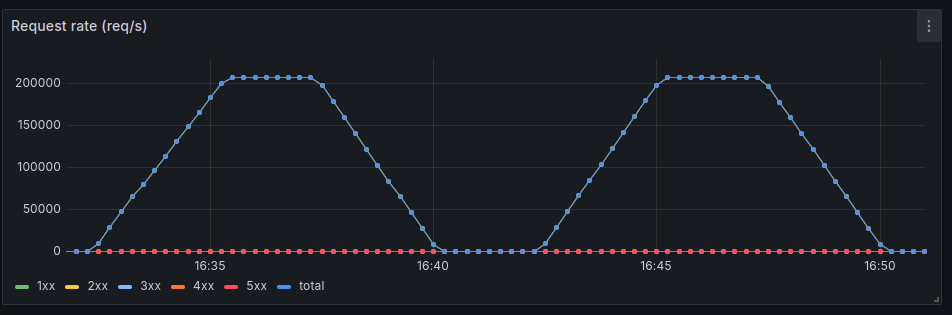
\includegraphics[scale=0.3]{chapter2/chap2-subfigure-example.png}
        \caption{Caption of figure 1}
        \label{fig:chap2-subfigure-example-1}
    \end{subfigure}%
    \begin{subfigure}{0.5\textwidth}
        \centering
        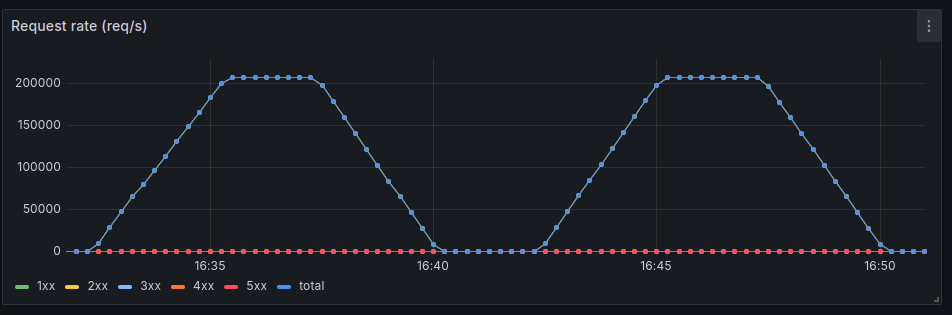
\includegraphics[scale=0.3]{chapter2/chap2-subfigure-example.png}
        \caption{Caption of figure 2}
        \label{fig:chap2-subfigure-example-2}
    \end{subfigure}
    \caption{Mô tả chèn hình ảnh con trong một hình ảnh lớn}
    \label{fig:chap2-subfigure-example}
\end{figure}

\section{Chèn hình ảnh toàn trang với ghi chú ở một bên}

% \begin{lstlisting}[language={[LaTeX]TeX}, caption={Chèn một hình ảnh vào báo cáo}, label={lst:figure}]
%     \begin{figure}[ht]
%         \begin{adjustbox}{addcode={\begin{minipage}{\width}}{\caption{%
%             Here is a caption of the figure which is so long that 
%             it has to be wrapped over multiple lines, but should 
%             not exceed the width (height after the rotation) of the image.
%             }\end{minipage}},rotate=90,center}
%             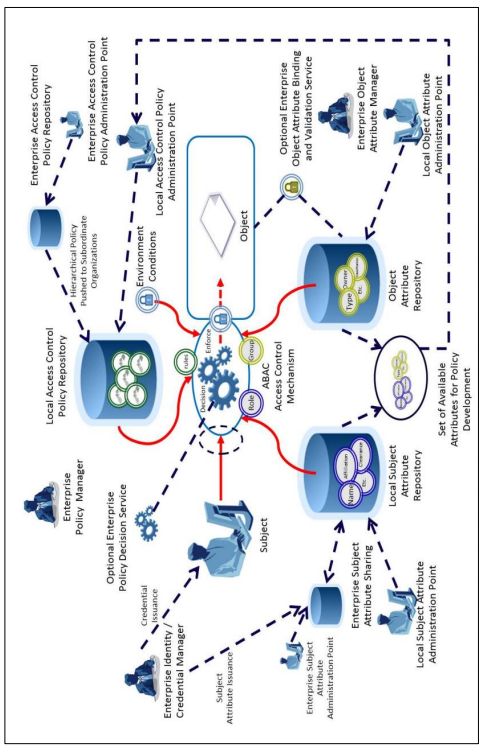
\includegraphics[scale=0.6]{chapter2/chap2-enterprise-abac.png}%
%         \end{adjustbox}
%       \end{figure}
          
% \end{lstlisting}

\begin{figure}[ht]
    \begin{adjustbox}{addcode={\begin{minipage}{\width}}{\caption{%
        Here is a caption of the figure which is so long that 
        it has to be wrapped over multiple lines, but should 
        not exceed the width (height after the rotation) of the image.
        }\end{minipage}},rotate=0,center}
        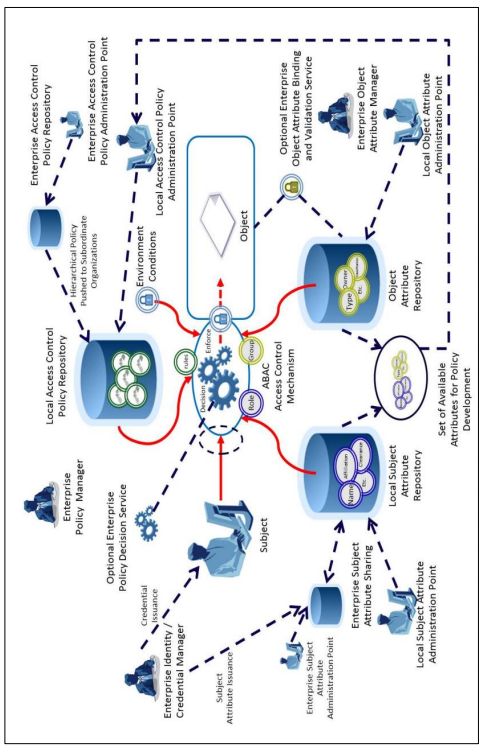
\includegraphics[scale=.6]{chapter2/chap2-enterprise-abac.png}%
    \end{adjustbox}
  \end{figure}